%\appendix
\begin{appendices}
\section{Matched Eigenfunction Expansion Method}
\label{sec:MEEM_details}
As introduced in section~\ref{sec:meem}, the hydrodynamic coefficients are computed semi-analytically using MEEM.
This section explains the MEEM formulation and solution methodology for the radiation of a dual truncated concentric cylinder geometry, originally presented in \cite{mavrakos_hydrodynamic_2004,chau_inertia_2010,chau_inertia_2012} as an extension of the single-cylinder MEEM radiation solution \cite{yeung_added_1981}.
Further numeric and realization details of the authors' implementation may be found in \cite{mccabe_investigating_2025,khanal_openflash_2025,mccabe_open-source_2024}.
The computation involves splitting the fluid domain into regions, approximating an infinite series by truncation, and solving a matrix equation to enforce the continuity of potential and velocity across regions. 

\subsection{Linear Hydrodynamics and Eigenfunctions}
The dynamics of a floating body in water waves are well-described by linear potential flow theory, a simplification of the Navier-Stokes equation.
This theory states that the fluid velocity field  is the gradient of some complex potential $\phi$, $\vec{v}=\nabla\phi$, and $\phi$ satisfies the Laplace equation, $\nabla^2\phi=0$.
Adding the free surface condition, far-field or incident waves, and body surface and sea-bed conditions detailed in \cite{chatjigeorgiou_analytical_2018} yields a boundary value problem.
When boundary conditions correspond to the heave radiation problem (body moving vertically, no incident waves), solving for the potential $\phi(r,\theta,z)$ determines the heave added mass and damping $A_h$ and $B_h$, hereafter ``hydro coefficients.”

For appropriate geometries, the partial differental equation is separable and $\phi$ can be expressed as the product of radial, vertical, and circumferential basis functions called eigenfunctions.
In cylindrically symmetric problems, the radial eigenfunctions are a family of transcendental functions called Bessel functions.
The fluid is then divided into cylindrical regions.
Arbitrarily many fluid regions can exist, so the method applies to any axisymmetric geometry, including multiple concentric bodies that oscillate independently.
Here, two concentric cylinders and thus three fluid regions are demonstrated.
Extension to many regions is discussed in section 3.4.
Figure~\ref{fig:meem-regions} illustrates the regions and dimensions: two internal regions \textit{i1} and \textit{i2}, and an external region \textit{e} extending to infinity.

\begin{figure}
    \centering
    \includegraphics[width=0.75\linewidth]{\matlabFilepath{27}}
    \caption{Fluid regions and dimensions used in the dual concentric cylinder MEEM}
    \label{fig:meem-regions}
\end{figure}

 The potential in each region is split into a homogeneous part for the unforced solution and a particular part due to body motion: $\phi=\phi_h+\phi_p$.
Boundary conditions dictate $\phi_p$ and the eigenfunctions for $\phi_h$ in each region, which the textbook \cite{chatjigeorgiou_analytical_2018} describes in detail.
Table~\ref{tab:MEEM-eigenfunctions} shows the equations originally presented in \cite{chau_inertia_2010,chau_inertia_2012} for the potential and eigenfunctions in each region, which include infinitely many unknown eigencoefficients $C_{1n}^{i1}$, $C_{1m}^{i2}$, $C_{2m}^{i2}$ and $B_{k}^{e}$.
By construction, this potential obeys all boundary conditions except for zero radial velocity on radial body surfaces.
The unknown coefficients must be computed to enforce this final condition as well as continuity across regions, which will be the subject of section \ref{sec:meem-matching}.

\begin{landscape}
\begin{table}
    \centering
    \begin{tabular}{|>{\centering\arraybackslash}p{0.085\linewidth}|>{\centering\arraybackslash}p{0.26\linewidth}|>{\centering\arraybackslash}p{0.34\linewidth}|>{\centering\arraybackslash}p{0.32\linewidth}|} \hline 
         Region&  $i1$&  $i2$& $e$\\ \hline 
         Homog. potential $\phi_h(r,z)$&  $\displaystyle\sum_n C_{1n}^{i1} R_{1n}^{i1}(r) Z_n^{i1}(z)$&  $\displaystyle\sum_m \left(C_{1m}^{i2} R_{1m}^{i2}(r) + C_{2m}^{i2} R_{2m}^{i2}(r) \right) Z_m^{i2}(z)$& $\displaystyle\sum_k B_k^e \Lambda_k(r) Z_k^e(z)$\\ \hline 
         Partic. potential $\phi_p(r,z)$&  $\displaystyle\frac{1}{2(h-d_1)}\left[ (z+h)^2 - \frac{r^2}{2}\right] $&  $\displaystyle\frac{1}{2(h-d_2)}\left[ (z+h)^2 - \frac{r^2}{2}\right]$& $0$\\ \hline 
         Radial eigen-function $R(r)$&  $R_{1n}^{i1}(r) = \begin{cases}
            \frac{1}{2} &  n=0 \\[1em]   %%% <--- here
            \frac{\mathrm{I}_0(\lambda_{n}^{i1}r)}{\mathrm{I}_0(\lambda_{n}^{i1}a_{2})} & n \ge 1
        \end{cases} $&  \shortstack{$R_{1m}^{i2}(r) = \begin{cases}
            \frac{1}{2} &  m=0 \\[1em]   %%% <--- here
            \frac{\mathrm{I}_0(\lambda_{m}^{i2}r)}{\mathrm{I}_0(\lambda_{m}^{i2}a_{2})} & m \ge 1
        \end{cases}$   \\ $R_{2m}^{i2}(r) = \begin{cases}
           \frac{1}{2}\ln(\frac{r}{a_2}) &  m = 0 \\
        \frac{\mathrm{K}_0(\lambda_{m}^{i2}r)}{\mathrm{K}_0(\lambda_{m}^{i2}a_{2})} & m \ge 1
        \end{cases}$}& $\Lambda_k(r) = \begin{cases}
           \frac{\mathrm{H}_0^{1}(m_0r)}{\mathrm{H}_0^{1}(m_0a_2)} & k = 0 \\[1em] 
          \frac{\mathrm{K}_0(m_kr)}{\mathrm{K}_0(m_ka_2)} &  k \ge 1
        \end{cases}$\\ \hline 
 Vertical eigen-function $Z(z)$& $Z_n^{i1}(z) = \begin{cases}
           1 & n=0 \\[1em]   %%% <--- here
           \sqrt{2}\cos(\lambda_{n}^{i1}(z+h)) & n \ge 1
        \end{cases}$& $Z_m^{i2}(z) = \begin{cases}
           1 & m=0 \\[1em]   %%% <--- here
           \sqrt{2}\cos(\lambda_{m}^{i2}(z+h)) & m \ge 1
        \end{cases}$&$    Z^{e}_{k}(z) = \begin{cases}
           N_0^{-\frac{1}{2}}\cosh( m_0(z+h)) &  k=0 \\[1em]   %%% <--- here
           N_k^{-\frac{1}{2}}\cos( m_k(z+h)) &  k \ge 1
        \end{cases}$\\ \hline
 Eigen-value& $\displaystyle \lambda_{n}^{i1} = \frac{n\pi}{h-d_{1}},  n \geq 1$& $\displaystyle \lambda_{m}^{i2} = \frac{m\pi}{h-d_{2}}, m \geq 1$&
 $\displaystyle \begin{cases} m_0 \tanh(m_0h)= \omega^2/g, & k=0 \\ m_k \tan(m_kh) = -\omega^2/g, & k \geq 1\\ \end{cases} $\\\hline
    \end{tabular}
    \caption{Equations for potential (homogeneous and particular) and eigenfunctions (radial and vertical) for each region.}
    \label{tab:MEEM-eigenfunctions}
  \fillandplacepagenumber
\end{table}
\end{landscape}

In Table~\ref{tab:MEEM-eigenfunctions},  $\textrm{I}_0$,  $\textrm{K}_0$, and $\textrm{H}_0^1$ are different Bessel functions of order zero; and 1M and 2M mean body 1 and 2 (spar and float) are moving respectively, while 1S and 2S mean each is stationary; and the $N_k$ expression is defined as:

\begin{equation}
    N_k = \frac{1}{2}\left(1+\frac{f_k}{2m_kh}  \right)~
    \textrm{ where }
    f_k = 
    \begin{cases}
        \sinh(2m_0h), & k=0 \\ \sin(2m_kh), & k\geq1
    \end{cases}
\end{equation}

 %%%%%%%%%%%%%%%%%%%%%%%%%%%%%%%%%%%%%%%%%%%%%%%%%%%%%%%%%%%%%%% begin equation helper functions %%%%%%%%%%%%%%%%%%%%%%%%%%%%%%%%%%%%%%%%%%%%%%%%%%%%%%%%%%%
%% integral definitions
\newcommand{\RintOneDefn}{
    \shortstack{
        $\displaystyle
            \boldsymbol{\mathcal{R}}_{1j} = 
            \int\limits_{a_{in}}^{a_{out}} \vec{R}_{1j}(r)r dr$ 
        \\
            for $j=(n,m)
        $
    }
}

\newcommand{\RintTwoDefn}{
    $\displaystyle \boldsymbol{\mathcal{R}}_{2m} = \int\limits_{a_{in}}^{a_{out}} \vec{R}_{2m}(r)rdr$
}

\newcommand{\ZmnDefn}{
    \shortstack{ 
        $\displaystyle \boldsymbol{\mathcal{Z}}_{nm} = \boldsymbol{\mathcal{Z}}_{mn}^T =$
        \\
        $\displaystyle \int_{-h}^{-d_1} \vec{Z}_n^{i1 ~T}\vec{Z}_m^{i2} dz$
    }
}
\newcommand{\ZmkDefn}{
    \shortstack{
        $\displaystyle \boldsymbol{\mathcal{Z}}_{mk} = \boldsymbol{\mathcal{Z}}_{km}^T = $
        \\
        $\displaystyle \int_{-h}^{-d_2} \vec{Z}_m^{i2 ~T}\vec{Z}_k^{e} dz $
    }
}

%% R definitions
\newcommand{\RintOneJzero}{
    $\displaystyle\frac{a_{out}^2-a_{in}^2}{4}$
}

\newcommand{\RintOneJOne}{
    $\displaystyle 
        \frac
            {a_{out} \mathrm{I}_1(\vec{\lambda}_j a_{out}) - a_{in}\mathrm{I}_1(\vec{\lambda}_j a_{in})}
            {\vec{\lambda}_j \mathrm{I}_0(\vec{\lambda}_j a_{scale})}
    $
}

\newcommand{\RintTwoJzero}{
    $\displaystyle
        \frac
        {
            f_{2m}a_{in}^2-a_{out}^2
        }
        {8}
    $
    where $
        f_{2m} = 1 + 2\ln\frac{a_{out}}{a_{in}}
    $
}

\newcommand{\RintTwoJOne}{
    $\displaystyle
    \frac
    {
        a_{in}\,\mathrm{K}_1 (
                \vec{\lambda}_m a_{in} )
        -a_{out}\,{\mathrm{K}}_1(
                \vec{\lambda}_m a_{out} )
    }
    {
        \vec{\lambda}_m \,{\mathrm{K}}_0 (
                \vec{\lambda}_m a_{scale} )
    }
    $
}

% Znm formulas
\newcommand{\ZnZeroMZero}{
    $h-d_1$
}

\newcommand{\ZnZeroMOne}{
    $\displaystyle
     \frac
                {\sqrt{2}\sin\left(
				\vec{\lambda}_m (h - d_1)
			\right)}
                { \vec{\lambda}_m}
    $
}

\newcommand{\ZnOneMZero}{
    $\displaystyle 0
     % this more complicated formula is only needed for multi-region
     %\frac
      %          {\sqrt{2}\sin(\vec{\lambda}_n^T (h - d_1))}
        %        { \vec{\lambda}_n^T}
    $
}

\newcommand{\ZnOneMOne}{
$\displaystyle
\begin{cases}
\frac{
            2 (-1)^{\vec{n}}
            }
            {
                    1 - \left(
                                    \frac{\vec{\lambda}_n^T}{  \vec{\lambda}_m}
                        \right)^2
            }
\frac{
            \sin\left(
                \vec{\lambda}_m(h-d_1)
         	\right)
            }
            {
            \vec{\lambda}_m
            }
,&  \lambda_n \neq \lambda_m\\
h -d_1, & \lambda_n = \lambda_m
\end{cases}
$
% this more complicated formula is only needed for multi-region
% \shortstack{
%     $\displaystyle
%     \frac
%         {\sin\left(
% 		(\vec{\lambda}_n^T + \vec{\lambda}_m)(h-d_1)
% 	\right)}
%         {\vec{\lambda}_n^T + \vec{\lambda}_m}
%     + Z_{nm}^-$
%     \\
%     where $Z_{nm}^-=
%     \begin{cases}
%         \frac
%             {\sin\left(
% 		(\vec{\lambda}_n^T - \vec{\lambda}_m)(h-d_1)
% 	\right)}
%             {(\vec{\lambda}_n^T - \vec{\lambda}_m)},
%         & \lambda_n \neq \lambda_m
%         \\
%         h-d_1,
%         & \lambda_n = \lambda_m
%     \end{cases}
%   $
%  }
}

% Zmk formulas
\newcommand{\ZmZeroKZero}{
    $\displaystyle \frac{\sinh(m_0(h-d_2))}{m_0 \sqrt{N_0}}$
}

\newcommand{\ZmOneKZero}{
    $\displaystyle \frac{\sqrt{2}~m_0 (-1)^{\vec{m}} \sinh(m_0(h-d_2))}{\sqrt{N_0} \left(m_0^2+{(\vec{\lambda}_m^T)}^2\right)}$
}

\newcommand{\ZkOneMZero}{
    $\displaystyle\frac{\sin(\vec{m}_k(h-d_2))}{\vec{m}_k \sqrt{\vec{N_k}}}$
}

\newcommand{\ZkOneMOne}{
    $\displaystyle
    \begin{cases}
            \frac{1}{\sqrt{2\vec{N_k}}}
            \left(
                \frac
                    {\sin\left((h-d_2)(\vec{m}_k+ \vec{\lambda}_m^T)\right)}
                    {\vec{m}_k+ \vec{\lambda}_m^T} + \right.
                 \\
                \left.~~~~~~~~~
                \frac
                    {\sin\left((h-d_2)(\vec{m}_k- \vec{\lambda}_m^T)\right)}
                    {\vec{m}_k- \vec{\lambda}_m^T} 
            \right),
        & |m_k| \neq \lambda_m
        \\
        \frac{h-d_2}{2},
        & |m_k| = \lambda_m 
    \end{cases}$
}

 %%%%%%%%%%%%%%%%%%%%%%%%%%%%%%%%%%%%%%%%%%%%%%%%%%%%%%%%%%%%%%% end equation helper functions %%%%%%%%%%%%%%%%%%%%%%%%%%%%%%%%%%%%%%%%%%%%%%%%%%%%%%%%%%%

Table~\ref{tab:meem-integrals} lists several integrals of the radial and vertical eigenfunctions, $\boldsymbol{\mathcal{R}}$ and $\boldsymbol{\mathcal{Z}}$ respectively, that will be needed in the calculations to follow. %\hl{Todo: need to define} $a_{scale}$.

\begin{landscape}
\begin{table}
    \centering
    \begin{tabular}{|c|c|>{\centering\arraybackslash}p{0.25\linewidth}|c|} \hline 
        \multicolumn{2}{|c|}{Integral}          & $m,j=0$           & $m,j\geq1$            \\ \hline 
        \multicolumn{2}{|c|}{\RintOneDefn}      & \RintOneJzero     & \RintOneJOne          \\ \hline 
        \multicolumn{2}{|c|}{\RintTwoDefn}      & \RintTwoJzero     & \RintTwoJOne          \\ \hline 
        \multirow{2}{*}{\ZmnDefn}   & $n=0$     & \ZnZeroMZero      & \ZnZeroMOne           \\ \cline{2-4} 
                                    & $n\geq1$  & \ZnOneMZero       & \ZnOneMOne            \\ \hline
        \multirow{2}{*}{\ZmkDefn}   & $k=0$     & \ZmZeroKZero      & \ZmOneKZero           \\ \cline{2-4}
                                    & $k\geq1$  & \ZkOneMZero       & \ZkOneMOne            \\ \hline
    \end{tabular}
    \caption{Eigenfunction integrals}
    \label{tab:meem-integrals}
    \fillandplacepagenumber
\end{table}
\end{landscape}

\subsection{Matching Across Fluid Boundaries}
\label{sec:meem-matching}

The eigencoefficients must be selected to enforce the radial velocity body boundary condition and the matching of the potentials and radial velocities at the edges of each region, earning this technique the name Matched Eigenfunction Expansion Method (MEEM).
The radiation problem was first solved this way for a floating cylinder in 1980 \cite{yeung_added_1981}.

First, the infinite sums in $\phi_h$ must be truncated.
Assuming truncation to $N$ terms in \textit{i1}, $M$ terms in \textit{i2}, and $K$ terms in \textit{e}, the total number of eigencoefficients to solve for is $N+2M+K$.
For a 3-region problem, there are 2 boundaries.
Thus there are four matching equations: (1) potential at $a_1$, (2) potential at $a_2$, (3) velocity at $a_1$, and (4) velocity at $a_2$.
As-is, this is not enough equations ($4 < N+2M+K$).
We must leverage eigenfunction orthogonality to get enough equations.
The first equation will turn into $N$ equations; the second and third each give $M$; the fourth $K$.
The transformation uses the following property of orthogonality.
Consider a generic function $Y(x)$ expressed as a series with coefficients $\alpha$ and basis functions $e(x)$: $Y(x)=\sum_i \alpha_i e_i(x)$.
If $e_j(x)$ is orthogonal to $e_i(x)$ from $x = a$ to $b$, then:

\begin{equation}
\begin{aligned}
       & \int\limits_a^b Y(x)e_j(x)dx = (b-a) <Y,e_j>=(b-a)<\sum_i \alpha_i e_i, e_j> \\ &= (b-a) \sum_i \alpha_i <e_i,e_j> = (b-a) \sum_i \alpha_i \delta_{ij} = (b-a) \alpha_j
\end{aligned}
\end{equation}

where $<\cdot,\cdot>$ is the inner product and $\delta_{ij}$ is Kronecker’s delta.
In the current hydrodynamics problem, the basis functions are the vertical eigenfunctions $Z_n^{i1}$, $Z_m^{i2}$, and $Z_k^{e}$.
Orthogonality of each eigenfunction can be verified with the inner product.
In the first region, for example, $<Z_{n_1}^{i1},Z_{n_2}^{i1}>=\delta_{n_1n_2}$.
Note that eigenfunctions of different domains are not orthogonal, and their inner products will be expressed as coupling integrals in \tableautorefname~\ref{tab:meem-integrals}.

For each of the four matching equations, the property of orthogonality applies only after multiplying by the appropriate eigenfunction and integrating over appropriate bounds.
For the potential matching equations, multiply both sides by the eigenfunction of the region with smaller fluid height (so $Z_n^{i1}$ at $a_1$ and $Z_m^{i2}$ at $a_2$).
Then integrate over that fluid height ($z=-h$ to $-d_1$ at $a_1$, and $-h$ to $-d_2$ at $a_2$).
For velocity matching, multiply instead by the eigenfunction corresponding to the larger region, while still integrating over the smaller region.
In velocity matching, an extra step is required to incorporate the boundary condition of zero radial velocity along the radial surface of the body.
Since it is zero-valued, the integral of this velocity may be added to one side of the equation (the one corresponding to the velocity of the larger region) to change the integration bounds only on that side.
This manifests in the bounds of the coupling integrals to be presented in \tableautorefname~\ref{tab:meem-integrals}.
Other combinations of eigenfunction multiplication or integration besides those described above are not useful since they result in integrating a quantity on a region where it is undefined, or a form unsuitable for the application of the orthogonality property.

\subsection{Block Matrix Structure}

Once orthogonality is applied, the matching equations create a linear system $A\vec{x}=\vec{b}$ where $A$ is a complex sparse $(N+2M+K)$x$(N+2M+K)$ square matrix corresponding to the homogeneous case, $\vec{x}=[\vec{C_{1n}^{i1}}, \vec{C_{1m}^{i2}}, \vec{C_{2m}^{i2}}, \vec{B_{k}^{e}}]$ is the complex eigencoefficient vector, and $\vec{b}$ is the real boundary condition vector corresponding to the particular case.
We elaborate on the block structure of the A-matrix and b-vector, an implementation detail that prior discussion of MEEM overlooks.
The A-matrix and b-vector block structures are shown in Tables~\ref{tab:MEEM-A-matrix} and \ref{tab:MEEM-b-vector} respectively.
They are written in compact notation using row vectors of basis functions, so $\vec{R_{1n}^{i1}}=[R_{10}^{i1}, R_{11}^{i1}, ..., R_{1(N-1)}^{i1}]$ and so on.
Each basis function is evaluated at the radius described to the left of its row in the table. $0_{ij}$ and $1_{ij}$ are the $i$ x $j$ matrices of zeros and ones respectively; diag($\cdot$) constructs a diagonal matrix from a vector; and $\odot$ is the Hadamard (element-wise) product.

\begin{landscape}
\begin{table}
    \centering
    \begin{tabular}{|>{\centering\arraybackslash}p{0.18\linewidth}|c||c|c|c|c|}\hline
 & & $\vec{C}_{1n}^{i1}$& $\vec{C}_{1m}^{i2}$& $\vec{C}_{2m}^{i2}$&$\vec{B}_k^e$\\\hline 
          &size&  N&  M&  M& K\\ \hline \hline 
          \shortstack{$\phi^{i1}=\phi^{i2}$ \\ at $r=a_1$}&N&  $(h-d_1)~\mathrm{diag}(\vec{R}_{1n}^{i1})$&  $-\boldsymbol{\mathcal{Z}}_{nm}\odot 1_{N1}\vec{R}_{1m}^{i2}$&  $-\boldsymbol{\mathcal{Z}}_{nm}\odot 1_{N1}\vec{R}_{2m}^{i2}$& $0_{NK}$\\ \hline 
          \shortstack{$\phi^{i2}=\phi^{e}$ \\ at $r=a_2$}&M&  $0_{MN}$&  $(h-d_2)~\mathrm{diag}(\vec{R}_{1m}^{i2})$&  $(h-d_2)~\mathrm{diag}(\vec{R}_{2m}^{i2})$& $-\boldsymbol{\mathcal{Z}}_{mk}\odot 1_{M1}\vec{\Lambda}_{k}$\\ \hline 
          \shortstack{$\frac{\partial}{\partial r}\phi^{i1}=\frac{\partial}{\partial r}\phi^{i2}$ \\ at $r=a_1$}&M&  $- \boldsymbol{\mathcal{Z}}_{mn} \odot 1_{M1} \frac{\partial}{\partial r}\vec{R}_{1n}^{i1}$&  $(h-d_2)~\mathrm{diag}(\frac{\partial}{\partial r}\vec{R}_{1m}^{i2})$&  $(h-d_2)~\mathrm{diag}(\frac{\partial}{\partial r}\vec{R}_{2m}^{i2})$& $0_{MK}$\\ \hline 
          \shortstack{$\frac{\partial}{\partial r}\phi^{i2}=\frac{\partial}{\partial r}\phi^{e}$ \\ at $r=a_2$}&K&  $0_{KN}$&  $-\boldsymbol{\mathcal{Z}}_{km} \odot 1_{K1}\frac{\partial}{\partial r}\vec{R}_{1m}^{i2}$&  $-\boldsymbol{\mathcal{Z}}_{km}\odot 1_{K1}\frac{\partial}{\partial r}\vec{R}_{2m}^{i2}$& $h~\mathrm{diag}(\frac{\partial}{\partial r}\vec{\Lambda}_k)$\\ \hline
    \end{tabular}
    \caption{MEEM A-matrix}
    \label{tab:MEEM-A-matrix}
      \fillandplacepagenumber
\end{table}
\end{landscape}
\begin{table}
    \centering
    \begin{tabular}{|c|c|} \hline 
         N& $\displaystyle
\int_{-h}^{-d_1} (\phi_p^{i2} - \phi_p^{i1})\vec{Z}_n^{i1~T} dz
$ \\ \hline 
         M& $\displaystyle-
\int_{-h}^{-d_2} \phi_p^{i2} \vec{Z}_m^{i2~T} dz
$\\ \hline 
         M& $\displaystyle
\int_{-h}^{-d_1} \frac{\partial}{\partial r}\phi_p^{i1}\vec{Z}_m^{i2~T} dz - \int_{-h}^{-d_2}\frac{\partial}{\partial r}\phi_p^{i2}\vec{Z}_m^{i2~T} dz
$\\ \hline 
         K& $\displaystyle
\int_{-h}^{-d_2} \frac{\partial}{\partial r}\phi_p^{i2} \vec{Z}_k^{e~T} dz
$\\ \hline
    \end{tabular}
    \caption{MEEM b-vector}
    \label{tab:MEEM-b-vector}
\end{table}

The dense blocks contain coupling integrals $\boldsymbol{\mathcal{Z}}$ of the vertical eigenfunctions.

Of the sixteen blocks that make up the matrix, six are diagonal, four are zero, and six are dense, resulting in the sparsity pattern shown in Figure~\ref{fig:sparsity}.
An even sparser matrix could be obtained with the alternate eigenfunction scaling for the second region described in \cite{chau_inertia_2012}. 
\begin{figure}
    \centering
    \includegraphics[width=0.75\linewidth]{\matlabFilepath{28}}
    \caption{A-matrix sparsity pattern, shown for $N=M=K=4$}
    \label{fig:sparsity}
\end{figure}


\subsection{Calculation of Outputs}

Once the eigencoefficients have been calculated by solving the linear system for $\vec{x}$, the hydrodynamic radiation coefficients $A_h$ and $B_h$ are found by integrating the potentials and velocities over the body surface:
\begin{alignat}{5}\label{eq:meem-c-derivation}
    A_h + \frac{iB_h}{\omega}&=\rho h^3  \int_{\theta=0}^{2\pi} & \int_{r=a_{in}}^{a_{out}} &\phi(r,z) \frac{\partial \phi(r,z)}{\partial z}r dr d\theta  \nonumber \\
    %
    %
    &= 2\pi \rho h^3 & \int_{r=a_{in}}^{a_{out}}&
   \left(\phi_p(r,z) + \sum_{j_1} C_{j_1} R_{j_1}(r)Z_{j_1}(z)\right) \nonumber \\
   %
  & & &  \left(\frac{\partial \phi_p(r,z)}{\partial z} + \sum_{j_2} C_{j_2} R_{j_2}(r)\frac{\partial Z_{j_2}(z)}{\partial z} \right)r dr \nonumber \\
    %
    %
    &= 2\pi \rho h^3 & \left[
    % first term
    \int_{r=a_{in}}^{a_{out}} \right. & \left.\phi_p(r,z)\frac{\partial \phi_p(r,z)}{\partial z} rdr  \right.
\\
    % second term
   & &  + \sum_{j_1} &C_{j_1} Z_{j_1}(z)\int_{r=a_{in}}^{a_{out}}R_{j_1}(r)\frac{\partial \phi_p(r,z)}{\partial z}rdr \nonumber \\
    % third term
    &&   + \sum_{j_2}& \frac{\partial Z_{j_2}(z)}{\partial z} C_{j_2}\int_{r=a_{in}}^{a_{out}}\phi_p(r,z)  R_{j_2}(r)rdr \nonumber \\
   % fourth term 
   & & +  \sum_{j_1}& \left.
C_{j_1}Z_{j_1}(z) \sum_{j_2} C_{j_2} \frac{\partial Z_{j_2}(z)}{\partial z}\int_{r=a_{in}}^{a_{out}} R_{j_1}(r)R_{j_2}(r)rdr\right] \nonumber
\end{alignat}
where the generic indices $j_1$ and $j_2$ are used to represent $n$ or $m$ depending on the region.
For regions with multiple radial eigenfunctions or surfaces covering multiple fluid regions, summation over each eigenfunction and region respectively is implied.
After substituting the eigenfunctions from Table~\ref{tab:MEEM-eigenfunctions} into \ref{eq:meem-c-derivation}, all $z$-dependent quantities are evaluated at the body draft on the integration surface, $z=-d$.
This means $\frac{\partial \phi_p}{\partial z}=1$, and $Z_j(z)$ simplifies to
\begin{equation}
    Z_j(z=-d) = \begin{cases}1,& j=0\\ \sqrt2(-1)^j,& j \geq 1\end{cases}
\end{equation}
The third and fourth integrals of \ref{eq:meem-c-derivation} vanish, and the second integral is the radial eigenfunction integral $\boldsymbol{\mathcal{R}}$ expressed previously in Table~\ref{tab:meem-integrals}. 

The first and second term are independent of and scale linearly with the eigencoefficients $\vec{x}$, respectively.
The radiation coefficients are thus computed as
\begin{equation}
    A_h + \frac{iB_h}{\omega}=2\pi \rho h^3(c_0 + \vec{c}\cdot\vec{x}) =2\pi \rho h^3(c_0 + \vec{c} \cdot A^{-1} \vec{b})
\end{equation}
with output constant $c_0$ and output row vector $\vec{c}$ defined as follows:
\begin{equation}
    c_0 =  \frac{\left({a^2_{out}}-{a^2_{in}}\right)\,\left(-{a^2_{in}}-{a^2_{out}}+4(h-d)^2\right)}{16\,\left(h - d\right)}
\end{equation}
\begin{table}[h]
    \centering
    \begin{tabular}{|l|c|c|c|c|} \hline 
          Body&N&  M&  M& K\\ \hline 
          Float&$0_{1N}$&  $\vec{Z}_m(z=-d) \odot\boldsymbol{\mathcal{R}}_{1m}$&  $\vec{Z}_m(z=-d) \odot\boldsymbol{\mathcal{R}}_{2m}$& $0_{1K}$\\ \hline
 Spar& $\vec{Z}_n(z=-d) \odot\boldsymbol{\mathcal{R}}_{1n}$& $0_{1M}$& $0_{1M}$&$0_{1K}$\\\hline
    \end{tabular}
    \caption{Output vector $\vec{c}$}
    \label{tab:MEEM-c-vector}
\end{table}
The appropriate dimensions are
\begin{equation}
    a_{out} = \begin{cases}
        a_2, & \text{float} \\
        a_1, & \text{spar}
    \end{cases} 
    \qquad
    a_{in} = \begin{cases}
        a_1, & \text{float} \\
        0, & \text{spar}
    \end{cases} 
    \qquad
   d = \begin{cases}
        -d_2, & \text{float} \\
        -d_1, & \text{spar}
    \end{cases} 
\end{equation}
to obtain the hydrodynamic coefficients of the float or the spar respectively.

Using the A-matrix and b- and c-vectors, the MEEM solution directly calculates radiation coefficients $B_h$ and $A_h$.
The hydrostatic stiffness $K_h$ and the excitation coefficient $\gamma$ are calculated as follows:
\begin{equation}\label{eq:gamma-K}
    |\gamma|  = \sqrt{\frac{ 4 \rho_w g V_g  B_h} {m_0}}, \quad % excitation
   \angle \gamma = -\frac{\pi}{2} + \angle\frac{ B_{k=0}^e}{\textrm{H}_0^{1}(m_0 a_2)},\quad
    K_h       = \rho_w g A_w  % hydrostatic stiffness
\end{equation}
where $g$ is the acceleration due to gravity, $\rho_w$ is the density of water, $m_0$ is the wavenumber, $V_g$ is the finite depth group velocity, $\textrm{H}_0^1$ is the zeroth-order Hankel function of the first kind, and $A_w= \frac{\pi}{4} D_f^2$ is the waterplane area \cite{newman}.
This method of calculating excitation from damping is the well-known Haskind relation.
Note that while the excitation magnitude $|\gamma|$ depends on the radiation damping $B_h$ which in turn depends on all the inner region eigencoefficients ($\vec{C}_{m}^{i2}$ for float excitation and $\vec{C}_{1n}^{i1}$ for the spar excitation), the excitation phase $\angle\gamma$ depends only on the first exterior eigencoefficient, $B_{k=0}^e$. 

\subsection{Validation}

Hydro coefficient results are validated by comparing to a benchmark shallow-water concentric-cylinder MEEM solution in \cite{chau_inertia_2012}.
Excellent agreement is observed, shown in Figure~\ref{fig:meem-yeung-validation}.
Authors of \cite{chau_inertia_2012} also experimentally validate their results in \cite{son_performance_2016}.
Previously in section~\ref{sec:meem}, the N=M=K=11 case was compared to WAMIT results for RM3 in deep water.

\begin{figure}
    \centering
    \includegraphics[width=0.75\linewidth]{\matlabFilepath{29}}
    \caption{Nondimensional added mass and damping coefficient validation against \cite{chau_inertia_2012}}
    \label{fig:meem-yeung-validation}
\end{figure}

\subsection{Convergence}

As $N,M,K\rightarrow\infty$, matching quality improves, and hydro coefficients converge toward their true values.
Previous MEEM papers use $N=M=K=50$ to obtain 4-digit matching accuracy without elaborating on convergence properties \cite{chau_inertia_2012}.
We observe that potential matching converges faster than velocity matching.
Figure~\ref{fig:meem-matching} shows the matching behavior for $N=M=K=11$, where potential matches well but velocity still has noticeable mismatch. 
\begin{figure}
    \centering
    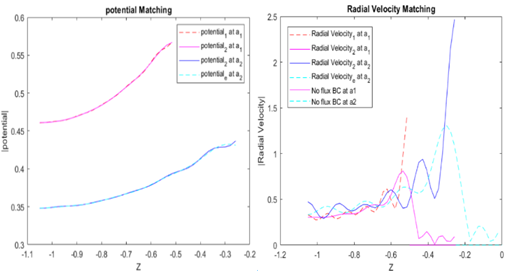
\includegraphics[width=0.75\linewidth]{figs/meem-matching.png}
    \caption{Matching for $N=M=K=11$ for benchmark geometry}
    \label{fig:meem-matching}
\end{figure}

Hydro coefficient convergence depends on the geometry: the benchmark shallow-water geometry of \cite{chau_inertia_2012} converges to within 0.25\% with only $N=M=K=4$, but RM3 requires $N=M=K>10$, shown in figure~\ref{fig:meem-convergence}.
There, damping converges well at low frequencies but requires more harmonics at higher frequencies, while added mass has similar convergence across frequencies. 
\begin{figure}
    \centering
    \includegraphics[width=0.75\linewidth]{\matlabFilepath{31}}
    \caption{Convergence for $N=M=K=(3,5,10,20)$ for RM3}
    \label{fig:meem-convergence}
\end{figure}


\subsection{Numerical Notes}\label{sec:meem-numerics}
Note that radial eigenfunctions $R_{1n}^{i1}(r)$ and $R_{1m}^{i2}(r)$ contain the modified bessel function of the first kind $\mathrm{I}_0(b)$, which diverges for $b\rightarrow \infty$.
This is the cause of the numeric overflow discussed in \ref{sec:meem}, where it was asserted that overflow occurs when the fluid region height to diameter ratio $\Delta z / D$ falls below some threshold.
The threshold is a function of the number of harmonics $N_{harmonics}$ used in that region ($N$ for spar, $M$ for float), as well as the maximum argument to the \texttt{besseli} function in MATLAB before overflow, $b_{max}$:
\begin{equation}\label{eq:delta-z-min}
    \frac{\Delta z_{min}}{D} = \frac{\pi N_{harmonics}}{2b_{max}} \approx \frac{N_{harmonics}}{446}.
\end{equation}
By trial, $b_{max}$ is found to be $\approx 700.5$, close to the theoretical value of \texttt{log(realmax)} $\approx 709.8$ for exponential scaling.
Since $N_{harmonics}=10$ gives adequate convergence for most geometries, this condition is trivially satisfied for nearly all floating bodies of practical relevance, but must still be added as a constraint to prevent the optimizer from exploiting the numerical divergence.
In future work, if high-accuracy solutions are desired for large bodies close to the sea floor, exponentially scaled bessel functions could be used instead, with symbolic cancellation of the exponential scaler from the eigenfunction numerator and denominator.

Likewise, the vertical eigenfunction $Z_k^e$ for $k=0$ contains the $\cosh$ and $\sinh$ functions, which diverge for large values of $m_0h$ (high frequencies or deep water).
Since the largest relevant value of $m_0h$ depends on the site rather than on the WEC design, it is not possible to add geometric constraints to prevent overflow as it was above.
Therefore, the limit is derived analytically. %\hl{This formula hasn't been numerically checked yet}
\begin{equation}
    \lim_{m_0h\rightarrow\infty} Z_0^e(z)= \frac{\cosh^2(m_0h)}{\sqrt{2m_0h}}\exp\left(1+\frac{z}{h}\right)
\end{equation}
Plugging this into the first element of the bottom block of the b-vector results in 
\begin{equation}
    \lim_{m_0h\rightarrow\infty}b_{N+2M+1}=\frac{-a_2}{h-d_2} \sqrt{\frac{h}{2m_0}}\exp(-d_2m_0)
\end{equation}
\begin{figure}
    \centering
    \includegraphics[width=.75\linewidth]{\matlabFilepath{32}}
    \caption{Asymptotic b-vector for large $m_0h$}
    \label{fig:meem-b-limit}
\end{figure}

%\hl{Todo: add sentence describing this figure and what it tells us}

And the corresponding limit for the vertical coupling integral:
\begin{equation}
\begin{aligned}
    \lim_{m_0h\rightarrow\infty}\boldsymbol{\mathcal{Z}}_{m,k=0} &
    %= \int_{-h}^{-d_2} \vec{Z}_m^{i2 ~T}\vec{Z}_0^{e} dz 
    = h~\frac{\cosh^2(m_0h)}{\sqrt{2m_0h}}\cdot \frac{-1+(-1)^m\exp(1-\frac{d_2}{h})}{f_{m}} \\
    \text{where}~~f_m&= \begin{cases}
        1, & m=0 \\
        h^2\lambda_m^2+1, & m \geq 1
    \end{cases}
    \end{aligned}
\end{equation}
%\hl{check this formula}

A final numerical subtlety worth discussing is finite precision effects in calculating $m_k$.
Bounds of $180^\textrm{o}\cdot[k-\frac{1}{2}, k]$ are placed on $m_kh$ in a root-finding algorithm to ensure the $k$th root is identified.
Degrees are used instead of radians so asymptotes occur at rational values.

\subsection{Runtime and Computational Cost Scaling}

The runtime of the MEEM method is the time required to find the eigencoefficients, then obtain the hydrodynamic coefficients from eigencoefficients.
First, a nonlinear root-finding algorithm runs $K-1$ times to generate the $m_k$ inputs used in the A-matrix and b-vector.
Then $3N+8M+2K-11$ Bessel functions must be evaluated for the radial terms of the A-matrix. % if I change scaling of i1 from a2 to a1, it reduces by N-1. if I change scaling of i2 from a2 to (a1+a2)/2, it increases by 2*(M-1). So total would be 2N+10M+2K-12. see notebook p51.
The cost of evaluating vertical coupling integrals (\tableautorefname~\ref{tab:meem-integrals}) is negligible since they are trigonometric.
Linear solves scale almost cubically with matrix size, so this step scales with $(N+2M+K)^3$.
The radial integrals for the c-vector do not require evaluating Bessel functions with any arguments that were not already evaluated for the A-matrix.
For $N=M=K=10$, the simulation averages \MEEMRuntime~ms on a Windows 10 laptop with a 2.5 GHz Intel i9 processor for a single frequency.
Figure~\ref{fig:runtime-hydro} shows the time breakdown.
Most of the time is spent evaluating Bessel functions, so future code optimization should focus on speeding up Bessel evaluations, such as with lookup tables.
\cite{chau_inertia_2012} proposes using the sparsity pattern to reduce matrix size from N+2M+K to 2M, but this seems low impact since the linear solve only takes a few percent of compute time.
On the other hand, matrix size in a boundary element method solver is much larger (meshes may have 1000s of panels) and the linear solve drives computation cost.
On the same machine, Capytaine boundary element method for the same geometry takes an average of 323 ms for a 710 panel mesh (1\% convergence).
Thus, MEEM achieves a 10x time reduction over Capytaine.

